\documentclass{article}
\usepackage{tikz}

\begin{document}

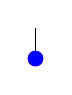
\begin{tikzpicture}
  \newcommand{\storeCoordinate}[3]{
    \pgfcoordinate{#1} at (#2,#3);
  }

  \storeCoordinate{myPoint1}{3}{4}
  \storeCoordinate{myPoint2}{-2}{1}

  \draw (0,0) -- (myPoint1);
  \node[circle, fill=red, inner sep=2pt] at (myPoint1) {};

  \draw (0,0) -- (myPoint2);
  \node[circle, fill=blue, inner sep=2pt] at (myPoint2) {};
\end{tikzpicture}

\end{document}